\chapter{Introduction}


To model environmental systems, data about the system  and resources to process this data to derive insight, is needed. Remote sensing data, such as satellite imagery and derived data products, such as land cover, vegetation indices, elevation models, or precipitation, are integral parts of environmental system models. 
The value of remotely-sensed data as a source of input data for environmental process modeling has been increasing in the past years (\cite{melesse2007remote}). The increasing availability of remotely-sensed data from different sensors with a wide range of spatial-, temporal- and radiometric-resolution has made remote sensing data, the best source of data for large-scale applications for a wide range of study fields like urban studies (\cite{wu2000global}), hydrological modeling (\cite{bogh2004incorporating}), watershed mapping (\cite{melesse2003spatially}), energy and water flux estimation (\cite{melesse2005estimation}), fractional vegetation cover (\cite{carlson2000impact}) and drought predictions (\cite{rhee2010monitoring}).

Through contributions of several earth observation missions, the stock of freely available remote sensing data, as well as its temporal- and spatial-resolution, is continuously growing (\cite{melesse2007remote}).
However, acquiring and preparing remotely-sensed data for the use as input for an environmental system model is still related to significant expenditures of time, expertise, work and processing resources. The reason for the necessary spending is strongly related to how remotely-sensed data is acquired, stored, managed and provided.

Most geospatial environmental data is derived from satellite imagery. This primary satellite imagery is retrieved from sensors of various earth observation satellite missions that, again, are part of mainly two earth observation programmes. The most extensive programme with regards to its duration and the number of satellites is the Earth Observing System (EOS). The EOS is a cooperation of National Aeronautics and Space Administration (NASA) including various Government Agencies such as the National Oceanic and Atmospheric Administration (NOAA) and the United States Geological Survey (USGS). The second observation programm is the recent Copernicus Programm of the European Commission in partnership with the European Space Agency (ESA; \cite{salomonson2002overview}). A representative satellite mission of the EOS is the Terra satellite that carries multiple sensors and among others produces the popular imagery products: Advanced Spaceborne Thermal Emission and Reflection Radiometer (ASTER) and Moderate-resolution Imaging Spectroradiometer (MODIS). The most well-known satellite missions are probably the Landsat satellites. The Copernicus Programm at the moment has two active missions: Sentinel 1 and Sentinel 2 (\cite{butler2014earth}).
From this primary satellite imagery, a multitude of secondary geospatial environmental data like Digital Elevation Models (DEMs), land cover, atmosphere, weather, climate simulations or even socio-economic variables are derived. Examples are the National Land Cover Database (NLCD) of the USGS, the NASS Cropland Data Layers of the National Agricultural Statistics Service (USDA) but also the WorldPop project population data produced by a collaboration between researchers at different Universities worldwide (\cite{homer2007completion},\cite{johnson20102009},\cite{tatem2017worldpop}). 
As a consequence of the decision of multiple U.S agencies including NASA, USGS and NOAA, as well as ESA to provide open access to their imagery data, petabyte-scale archives of geospatial data are now freely available (\cite{gorelick2017google}).

Usually, the databases are accessible through an online search and order tool like the NASA Earth Observation, the USGS Earth Explorer or the Copernicus Open Access Hub. These tools allow searching for scenes of a remote sensing data product according to different metadata properties like acquisition time, name or spatial-coverage and order or download the selected scenes subsequently. 
Scenes are near-square images covering an area that varies in size depending on the remote sensing data. For Landsat images, the coverage is about 170 to 185 km per scene. Because these online search and order tools do not provide any processing resource, it is not possible to aggregate or subdivide the scenes to a specific extent.

\begin{center}
	\begin{figure}[h]
		\begin{center}
			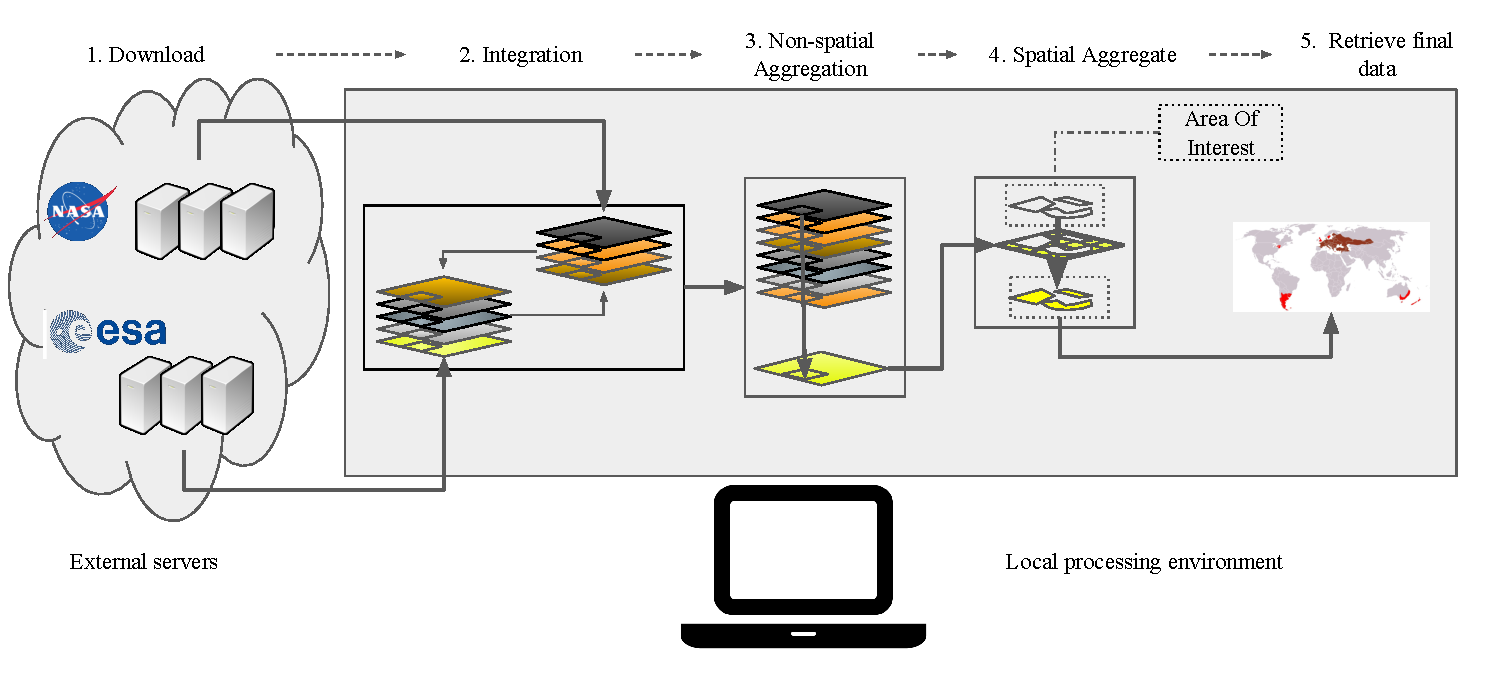
\includegraphics[width=15cm]{images/traditional_acquisition-cropped.pdf}
			\caption{Schematic approach to acquire and prepare remote sensing data for environmental system modeling}
			\label{traditionl_approach}
		\end{center}
	\end{figure}
	% \vskip 2em%
\end{center}


A standard procedure of acquiring and preparing remote sensing data comprises several steps. First, the remote sensing data must be downloaded via one of the search and order tools. If the downloaded data is acquired from multiple sensors or different sources, the different coordinate reference systems and projections need to be integrated and harmonised. Third, in case of multiple scenes of the same locations, for instance, multiple satellite images of the same location acquired at different times, the data has to be aggregated temporally. For example to calculate the yearly sum of precipitation from daily chirps satellite imagery, or to calculate the Normalised Diference Vegetation Index (NDVI) from multiple bands of Landsat imagery.
Forth, the data is spatially aggregated according to a given target. The target represents the shape of the area of interest (AOI). The AOI could be a world-wide grid of 1$^\circ$ x 1$^\circ$ cells, the resolution of a raster, a set of points representing the locations of experiments, or the sample area. Finally, in the last step, the data is retrieved as tabular data with a geographic reference (see Figure \ref{traditionl_approach}). The entire processing of the remote sensing data was performed on the local system.

The standard procedure to acquire remote sensing data is usually time consuming and cumbersome due to the interoperability and size of remote sensing data (\cite{iosifescu2011geovite}).

Because varies governments and agencies collect remote sensing data, most data are distributed and stored in different locations, in a variety of file formats, projections and resolutions. To integrate data from such diverse sources requires a manual and thus time-consuming pre-processing of the data even when processing only a few satellite images (\cite{schell2000geodata}). To perform the required integration and harmonisation of different remote sensing data sets expertise in a Geographic Information System (GIS) is prerequisite.

Furthermore, due to the limited possibility of the search and order tools to control the request to the servers, the data throughput is unnecessary high. Even though only a fraction of a scene is needed, the complete scene needs to be downloaded. Furthermore, the processing resources are not where they are needed. It is required to download the entire row data to a local system to perform the tasks necessary to prepare the data for environmental modeling. The limited control over the requested data results in many unnecessary inter-products and again raises the data throughput. While processing small geospatial data sets, this may be of no importance, but for the processing of large-scale data sets, this quickly leads to challenges in dealing with memory limitation and the necessity for big data solutions such as computer clusters or cloud computing resources.
Managing such application leads to associated challenges such as storage, management of databases and servers and managing clusters efficiently (\cite{gorelick2017google}). 

For instance, the processing of a moderately sized remote sensing imagery stack with 50 landsat satellite images (1.6 GB per image) would most likely lead to a memory limitation problems.

Hence, although petabyte-scale archives of geospatial data are freely available, the access and utilisation of these datasets for environmental system modelling are restricted due to the given difficulties. 
These obstacles hinder most researchers to make use of this massive stack of remote sensing imagery, restricting access to the information that can be derived from large remote sensing datasets, to remote-sensing experts with exclusive access to high-performance computing resources.



\subsection{The potential of the GEE for the acquisition of remote sensing data}

The EE thus offers an elegant solution for working with large remote sensing data and the related problems of the interoperability of the data due to distributed sources and the big data problems caused by the size of the data and required processing resources. 
Processing resources and data are connected, and there are no unnecessary inter-products or downloads. 
The data does not have to be download and preprocessed separately. Instead, the data is already stored in one managed database, pre-processed and in access and analysis-ready format. 
The computational power required to process the data is automatically scaled, which makes computations of an entirely new magnitude possible without bothering with any IT management obstacles.
With EE, it is possible to request and generate precisely the data needed for analysis, while any acquisition, integration, preprocessing and aggregation is outsourced to the EE servers. 

However, the EE API is controlled by a client library, currently only available in JavaScript and Python. To use the EE additional effort to learn and apply the client libraries is necessary, furthermore, scientists using a different programming language like R cannot access the EE API directly from within R.
There is currently no R or Python package that is using EE capabilities to simplify the acquisition and preprocessing of remotely sensed data. Actually, there is not a single R or Python package using any of EE capabilities directly. The few existing ones are written in Python and only facilitate the use of the EE API by providing a pipeline to other API's like the Planet-GEE-Pipeline-GUI or provide an automated upload feature of assets via the Google Cloud Environment like the geeadd tool (\cite{roy2017google}).

In summary, although the Earth Engine solves many of the challenges in retrieving data from large remote sensing datasets for environmental system modeling, it is still exclusive for experienced users of the EE client library available only in JavaScript and Python.

\section{The earthEngineGrabR}

To recap the current situation:
\begin{itemize}
	
	\item The stack and resolution of freely available remote sensing data, as the potential as input for environmental system model, is continuously increasing.
	\item With the traditional methods discussed, the process of acquiring remote sensing data for analysis is costly and inefficient and requires high-performance computing resources.
	\item This restricting access to the information that can be derived from large remote sensing datasets, to remote-sensing experts and deviates resources from the scientific work.
	\item The EE provides a performant and flexible solution to the problems related to large remote sensing datasets and is superior to the acquisition with a search and order tool.
	\item However, the use of the EE is exclusive for experienced users of the EE client library only available for Python.
	\item Hence, to use the potential of the EE for the acquisition of remote sensing data, the access to the EE needs to be simplified.
	
\end{itemize}

The simplified access to the capabilities of EE would enable scientists to utilise the massive stack of freely available remote sensing data for their research projects without additional costs.

This work is inspired by the attempt to develop such simplified access to capabilities of the EE for the R programming environment.

The master's thesis aims is to develop an R package - the earthEngineGrabR, which simplifies the acquisition of remote sensing data for the analysis in R. This should be accomplished by building an interface between R and EE.
The interface should enable to use EE as a backend-service to retrieve selected data sets for a given region and time of interest in an analysis-ready format. The interface is supposed to extract data from the EE data catalogue while providing extensive control over temporal and spatial resolution. 
Any processing of the remote sensing data shall entirely be outsourced to the EE and only the derived data products, are exported from EE and imported in R. 

This way, the developed interface exploits two of EE's significant advantages. One is the public data catalogue of over 11 petabytes of remote sensing data in an analysis-ready format, and the other is its high-performance, intrinsically parallel computation service to process such massive data.





\section{Introduction to Google Earth Engine}

EE is a cloud-based platform that strongly simplifies the access to high-performance computing resources to process extensive remote sensing datasets, without the information technology (IT) management obstacles like, data acquisition and storage, combine different file formats, managing databases, machine allocations, CPUs, GPUs. 
EE consists of a multi-petabyte data catalogue, a high performance, parallel and therefore scaleable, computation service and is accessed and controlled through an Internet-accessible application programming interface (API). Queries are constructed by using operations drawn from the Earth Engine client library consisting of more than 800 functions ranging from simple mathematical operations to powerful geostatistical, machine learning and image processing operations (\cite{gorelick2017google}).

\subsubsection{The public data catalogue}

The majority of the EE public data catalogue consists of remote sensing imagery collected by earth-observing satellites missions from government agencies like NASA, USGS, NOAA and ESA. It contains the entire archives of Landsat, Sentinel 1-2 and Modis, but also several other environmental, geophysical and social-economic datasets. This catalogue is continuously extended and updated from current missions, and this way holds up to date satellite imagery with a latency of about one day.
In EE, imagery data or raster is stored in a 2D gridded raster container referred to as an image. One image can have any number of bands, and while each band need to be homogeneous in data type, resolution and projection, bands in an image can vary in data type, resolution and projection. Each image can have associated metadata stored as key-value pairs to provide additional information like acquisition time, location or any metadata provided.
Multiple images that are related, such as images from the same source or sensor are combined in collections. These Collections provide fast spatial and temporal filtering and sorting capabilities using metadata associated to every single image in the collection. The metadata enables users to search through millions of images to select data that meet specific criteria. For example, users can quickly filter the entire Landsat 7 archive for images within Germany, collected on day-of-year 40 - 80, from the year 1990 - 2000 with cloud cover less 50\%. While this also would be possible in one of the search and order tools, EE additionally provides extensive GIS capabilities and processing resources to further manipulate the data.
For instance, the filtered Landsat scenes could be aggregated to a median composite. The bands in the median composite could be used to calculate the Normalized Difference Vegetation Index (NDVI). The NDVI image could be spatially aggregated over multiple regions defined by the feature of a shapefile representing the states of Germany. While this process is a matter of minutes on Earth Engine, it indeed would require extended big data solutions on a local system.

What makes EE that performant is the storage system as a tile database with built-in pyramiding architecture in combination with the system architecture and several data distribution models (\cite{gorelick2017google}).

\subsubsection{The tile architecture}

Images ingested into Earth Engine are preprocessed to provide fast and efficient access. First, images are parsed into tiles in the images original projection and resolution and stored in a tile database. Each tile has the size of 256 x 256 Pixels and refers to the practical trade-off between loading unneeded data versus the overhead of issuing additional reads. Instead of resampling all data to a fixed grid, traditional data cube systems would do, this method is information-preserving (\cite{gray1997data}). Because the data is maintained in their original projection, resolution and bit depth the data degradation that is inevitable if resampling to a fixed grid, is avoided

\subsubsection{The pyramid architecture}

Additionally, a pyramid of reduced-resolution tiles is created for each image and stored in the tile database. Each level of the pyramid is produced by downsampling the previous level by a factor of two until the entire image fits into a single tile. During downsampling, continuous valued bands by default are averaged, while discrete-valued bands are aggregated using one of min, mode, max. This way, if fractions of data from an image are requested for computation in a reduced resolution, only the relevant tiles from the most appropriate pyramid level need to be retrieved from the tile database. The tile database enables EE to provide data in a variety of resolutions without introducing significant storage overhead.

\subsubsection{The system architecture}

The processing system automatically subdivides and distributes computations to enable high-throughput analysis. In EE a collection of enabling technologies is used that is available in the Google data centre environment. The Borg Cluster Management System is used to distribute and load-balance computation over multiple workers within a cluster. The FlumeJava framework is used for parallel pipeline execution of batch computations.
Users can interact with the Earth Engine by using either an associated web-based interactive development environment (IDE), third-party Web Apps, or directly with one of the client libraries on a local system by using the EE Python or JavaScript API.
The IDE code editor and the third-party Web Apps use the client libraries to send requests to EE through a Representational State Transfer Application Programming Interface (REST API). 
The Tilestore Servers houses the public data catalogue in the described architecture. In the Asset Database, the user can ingest their data. 
The Borg Cluster Management Software manages each component of the system, and each service is load-balanced over multiple workers. Failure of any individual workers results in the caller reissuing the query.

\subsubsection{Construct earth engine programmes with the client library}

The user writes EE programmes using the client library available for Python and JavaScript.
The functions in the client library can be composed to build a description of the computation the user wants to perform. This description is sent to Earth Engine servers for evaluation. To further improve performance Earth Engine uses a lazy evaluation model that allows it to compute only the fraction of output that is necessary to fulfill the current request. It postpones computing output pixels until it knows more about the context in which they are needed (\cite{gorelick2017google}).


\subsubsection{Data distribution models}

To achieve high performance, the functions in the Earth Engine library apply several built-in parallelisation and data distribution models. Each model aims to optimise a different data access pattern.
For operations that are local, image tiling is used.
In remote sensing, especially raster manipulation many processing operations are local. That is, the computation of a Pixel depends only on input pixels within a fixed distance. Examples of per-pixel operations are band math, spectral unmixing neighbourhood or convolution operations. To process operations in parallel, the area is subdivided into tiles and computed independently. This way, to process one of those tiles most of the time only a few or one input tile is needed. Image tiling combined with pyramided inputs provides a fast computation of results at any requested scale or projection.
For operations that are inherently non-local a spatial aggregations is used.
Non-local operations such as computations of regional or global statistics, raster-to-vector conversions, or sampling an image to train a classifier, can at least partly still be executed in parallel by aggregating together many sub-results. In EE, those processes are executed as distributed processes using a scatter-gather model. First, similar to the image tiling approach, a spatial region is divided into subregions that are allocated to workers in a distributed worker pool and computed independently. These intermediate results are sent back to the master of this computation, which combines them and transform the intermediate results into the final result. For instance, to compute a mean value each worker computes sums and counts, the master collects these intermediate results and compute the final results as the total sum by the total count.



